% Template for ICIP-2013 paper; to be used with:
%          spconf.sty  - ICASSP/ICIP LaTeX style file, and
%          IEEEbib.bst - IEEE bibliography style file.
% --------------------------------------------------------------------------
\documentclass{article}
\usepackage{spconf,amsmath,graphicx}


% Example definitions.
% --------------------
\def\x{{\mathbf x}}
\def\L{{\cal L}}

% Title.
% ------
\title{Investigation on convergence of Neural Network Training using Butterfly mixing}
%
% Single address.
% ---------------
\name{Haoyu Chen (SID:23269048)$^1$}
\address{$^1$ Dept. of Electrical Engineering \& Computer Science, University of California, Berkeley, CA, USA \\
{\small \tt \{haoyuchen@berkeley.edu\}}
}
%
% For example:
% ------------
%\address{School\\
%	Department\\
%	Address}
%
% Two addresses (uncomment and modify for two-address case).
% ----------------------------------------------------------
%\twoauthors
%  {A. Author-one, B. Author-two\sthanks{Thanks to XYZ agency for funding.}}
%	{School A-B\\
%	Department A-B\\
%	Address A-B}
%  {C. Author-three, D. Author-four\sthanks{The fourth author performed the work
%	while at ...}}
%	{School C-D\\
%	Department C-D\\
%	Address C-D}
%
\begin{document}
%\ninept
%
\maketitle
%
\begin{abstract}
In this project, I investigate the convergence of training neural networks (NN) by butterfly mixing and all-reduce data communication styles. The system is built on single machine to simulate the distributed system to train the NN. Data is partitioned to different threads for local model update. Model averaging (reduce) is done every few minibatches. I compare two different reduce strategies: all reduce, and butterfly mixing. We show that butterfly can be a possible candidate to be utilized in real distributed system to speed up the traning process.

\end{abstract}
%
\begin{keywords}
neural network, butterfly mixing, convergence analysis
\end{keywords}
%
\section{Introduction}
\label{sec:intro}

Deep Neural Networks (DNN) has shown its effeciveness in several machine learning tasks. The large model size and massive training examples make DNN a powerful model for classification. However, these two factors also slow down the training procedure of DNNs.

Parallelization of DNN training has been a popular topic since the revive of neural networks. Several different strategies have been proposed to tackle this problem. Multiple thread CPU parallelization and single CUDA GPU implementation are compared in \cite{scanzio2010parallel,vesely2010parallel}, and they show that single GPU could beat 8 cores CPU by a factor of 2. However, for a real big data problem, single machine is not powerful enough to train the model. Thus, the distributed system is applied to tackle this problem.

Optimality for parallelization of DNN training was analyzed in \cite{seide2014parallelizability}, and based on the analysis,a gradient quantization approach was proposed to minimize communication cost \cite{seide20141}.

With distributed system, one of the key issue is to minimize the network communication. The most common message collection strategy is all-reduce, which reduce the weight from all the nodes, average the weights, and boardcast the averaged weights to all the nodes at each update. This method can collect and boardcast information completely, but it requires large bandwidth, and its communication is quite heavy. Butterfly mixing was proposed in \cite{zhao2013butterfly} to interleave communication with computation for convex optimization problem. Butterfly mixing can diminish the communication among the nodes in the network with sacrificing the amount of message communication. However, the non-convex optimization problem is much more complex than convex optimization, it is questionable whether the butterfly mixing strategy can achieve the fast convergence for training DNN.

In this project, I focus on investigating the convergence of training NN by butterfly mixing communication strategy. For simplification, I use a single machine to simulate the distributed system, thus, I do not try to build a parallel system. I implement a simple neural network, and a system to simulate the distributed system for single machine. The analysis results can help people decide whether to apply butterfly mixing to speed up the DNN training process in a distributed system.

In Sect 2, the details of my deep neural network is introduced. In Sect 3, I explain the reason why I choose to communicate the weight rather than the gradient of weights. In Sect 4, the reduce strategies are shown. In Sect 5, the results are analyzed.  

\section{Neural network setup}

The neural network is implemented in MATLAB. It has one input layer, arbitrary number of hidden layer, and one softmax output layer, see Fig.~1. Between each layer, the nodes are fully connected. The activation function I chose is ReLu, which can keep the gradient in a resonable value for NN. I initialize the weight matrix randomly.

\begin{figure}[h!]

  \centering
    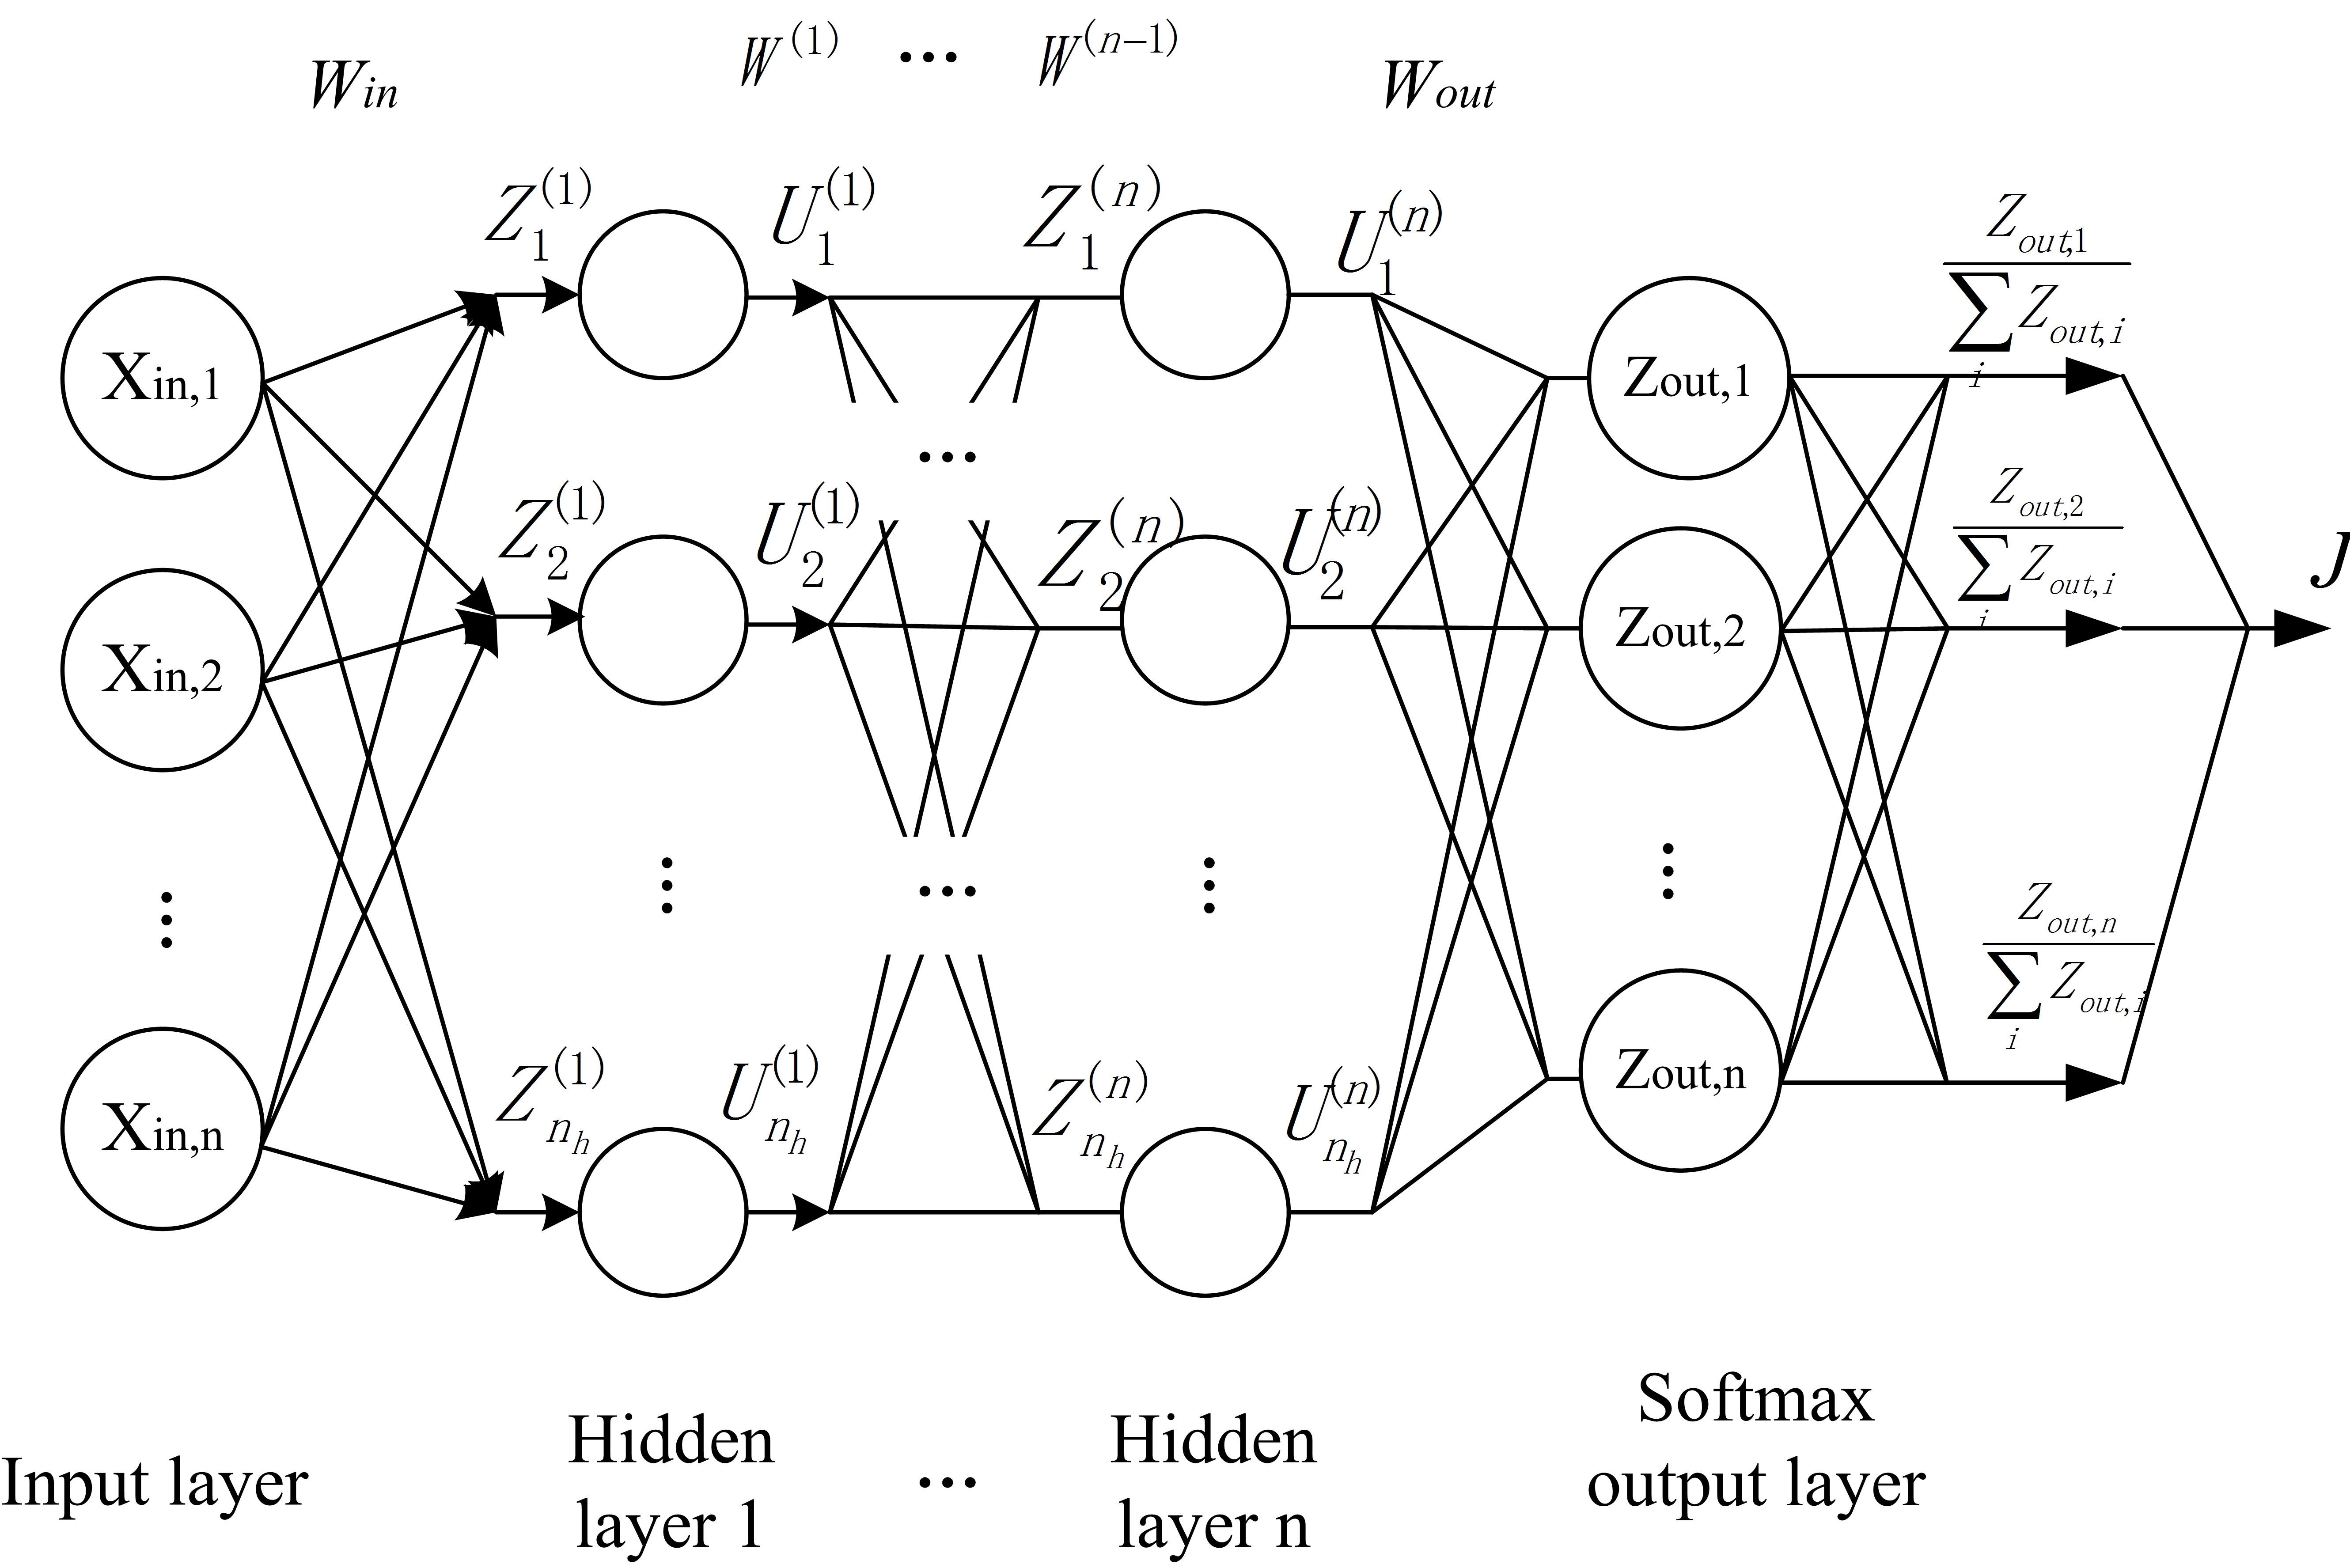
\includegraphics[width=0.45\textwidth]{cs289_6.jpg}
  \caption{network structure}
\end{figure}

\section{Data parallelization and Model Averging}
Gradient descent method is applied to train the DNN model even it's a non-convex optimization problem. Since the size of training data is large, batch training is applied to approximately compute the gradient for each iteration. Rougly, the larger batch size, the higher converge speed. However, the large batch size brings the computing time and memory usage problem. With using distributed system, the gradient can be computed at each node, communicate among all the nodes, and average recieved gradient at each update iteration. This method can compute the reduced gradient accurategly, but it requires heavy communication, since we need to communicate at each update iteration. \\

However, if the weight rather than gradient of weight is choosen to reduce and average, it is not necessary to communicate the weight at each iteration for incomplete message communication. However, for the all-reduce, it is the equvalent as communication the gradients of weight, if the update method is just simple batch gradient update. In this project, I choose to communicate the weight for some fixed iterations steps, so that frequency of communication do not have to be too high.

\section{Convergence Analysis}
\cite{zhao2013butterfly} provides a convergence analysis for convex optimization problem, however, their proof is incorrect. In this section, we prove the convergence of distributed convex optimization with any communication strategy if they pass messages to all the node in $log(N_{node})$ steps, where $N_{node}$ is the number of nodes in the system.\\

\cite{parallelDistCom} provides a general proof for distributed stochastic gradient algorithms. Our proof is based on their general proof. Generally our problem can be formulated as: \\
\[x^i(t+1) = \sum_{j|t \in T^{ij}} a^{ij}(t)x^j(\tau^{ij}(t)) + \gamma^i(t)s^i(t)\]
where $t$ is the time; $\tau^{ij}(t)$ is the time at which the message $x_l^j$ (received by $i$ at time $t$) was transmitted by processor $j$; $T^{ij}$ is the set of times that such a message is received by processor $i$ from processor $j$; $x^i(t)$ is the message received by $i$ at time $t$; $s^i(t)$ is the gradient computed by processor $i$ at time $t$; $\gamma^i(t)$ is the parameter corresponding to $s^i(t)$; and $a^{ij}(t)$ are nonnegative scalar coefficients for $x^i(t)$. $a^{ij}(t)$ satisflies $\sum_{j|t \in T^{ij}}a^{ij}(t) = 1$.\\

This formular can be re-writed as:\\
\[x^i(t) = \sum_{j=1}^p \Phi^{ij}(t,0)x^j(1) + \sum_{\tau = 1} ^{t-1} \sum_{j=1}^p \Phi^{ij}(t,\tau)\gamma^j(\tau)s^j(\tau)\]
where $\Phi^{ij}(t,\tau)$ depends on the particular realization of the communication algorithms. It represents the cumulative strength of message from thread $j$ to thread $i$ sended at time $\tau$, received at time $t$.    \\

\cite{parallelDistCom} proves that if the condition hold below, the problem can be converged in XXX\\
\[|\Phi^{ij}(t,\tau) - \Phi^j(\tau)|\leq A\rho^{t-\tau}, \forall t> \tau\leq0\]

We prove that $|\Phi^{ij}(t,\tau) - 0|\leq A\rho^{t-\tau}, \forall t> \tau\leq0$ holds if the message from one node will be passed to all the nodes in the network within $log(N_{node})$ iterations. Let's set the time when a message (notated as $m$) is generated by a node be $t_0$. Since each node only send the integrated message to one other node and each node only recieves one message from another node, $a^{i,j}(t) = 0.5 \forall i,j,t$. Thus, before $t_0 + log(N_{node})$ iterations, the sum of the weight for $m$ though all the network is 1. However, after $t_0 + log(N_{node})$, the sum of the weight for $m$ reduce by half for each iteration, since the number of the node in the network is fixed, and $m$ has reached all the nodes in the network. Thus, $|\sum_{i}\Phi^{ij}(t,\tau) - 0|\leq A\rho^{t-\tau}, \forall t> \tau\leq0$. Since the $\Phi$ is nonnegative scales, $|\Phi^{ij}(t,\tau) - 0|\leq A\rho^{t-\tau}, \forall t> \tau\leq0$ holds.   
\section{Different Reduce Strategies}
In this section, the two data reduce strategies are introduced, which are all-reduce, and butterfly mixing.

 \subsection{All-reduce}

All-reduce startegy collects the weights from all the nodes in the network. The communication is bounded by the bandwidth. Fig.~2 is an example of all-reduce with 4 nodes. After one node collects all the weights, it will average the weights and then boardcast it too all the nodes. Thus, the all-reduce requires at least twice communication to collect and boardcast the messages. However, the all-reduce can compute the average weight based on full information for the whole network. Thus, the converge speed of all-reduce should be the fastest.
\begin{figure}[h!]
  
  \centering
    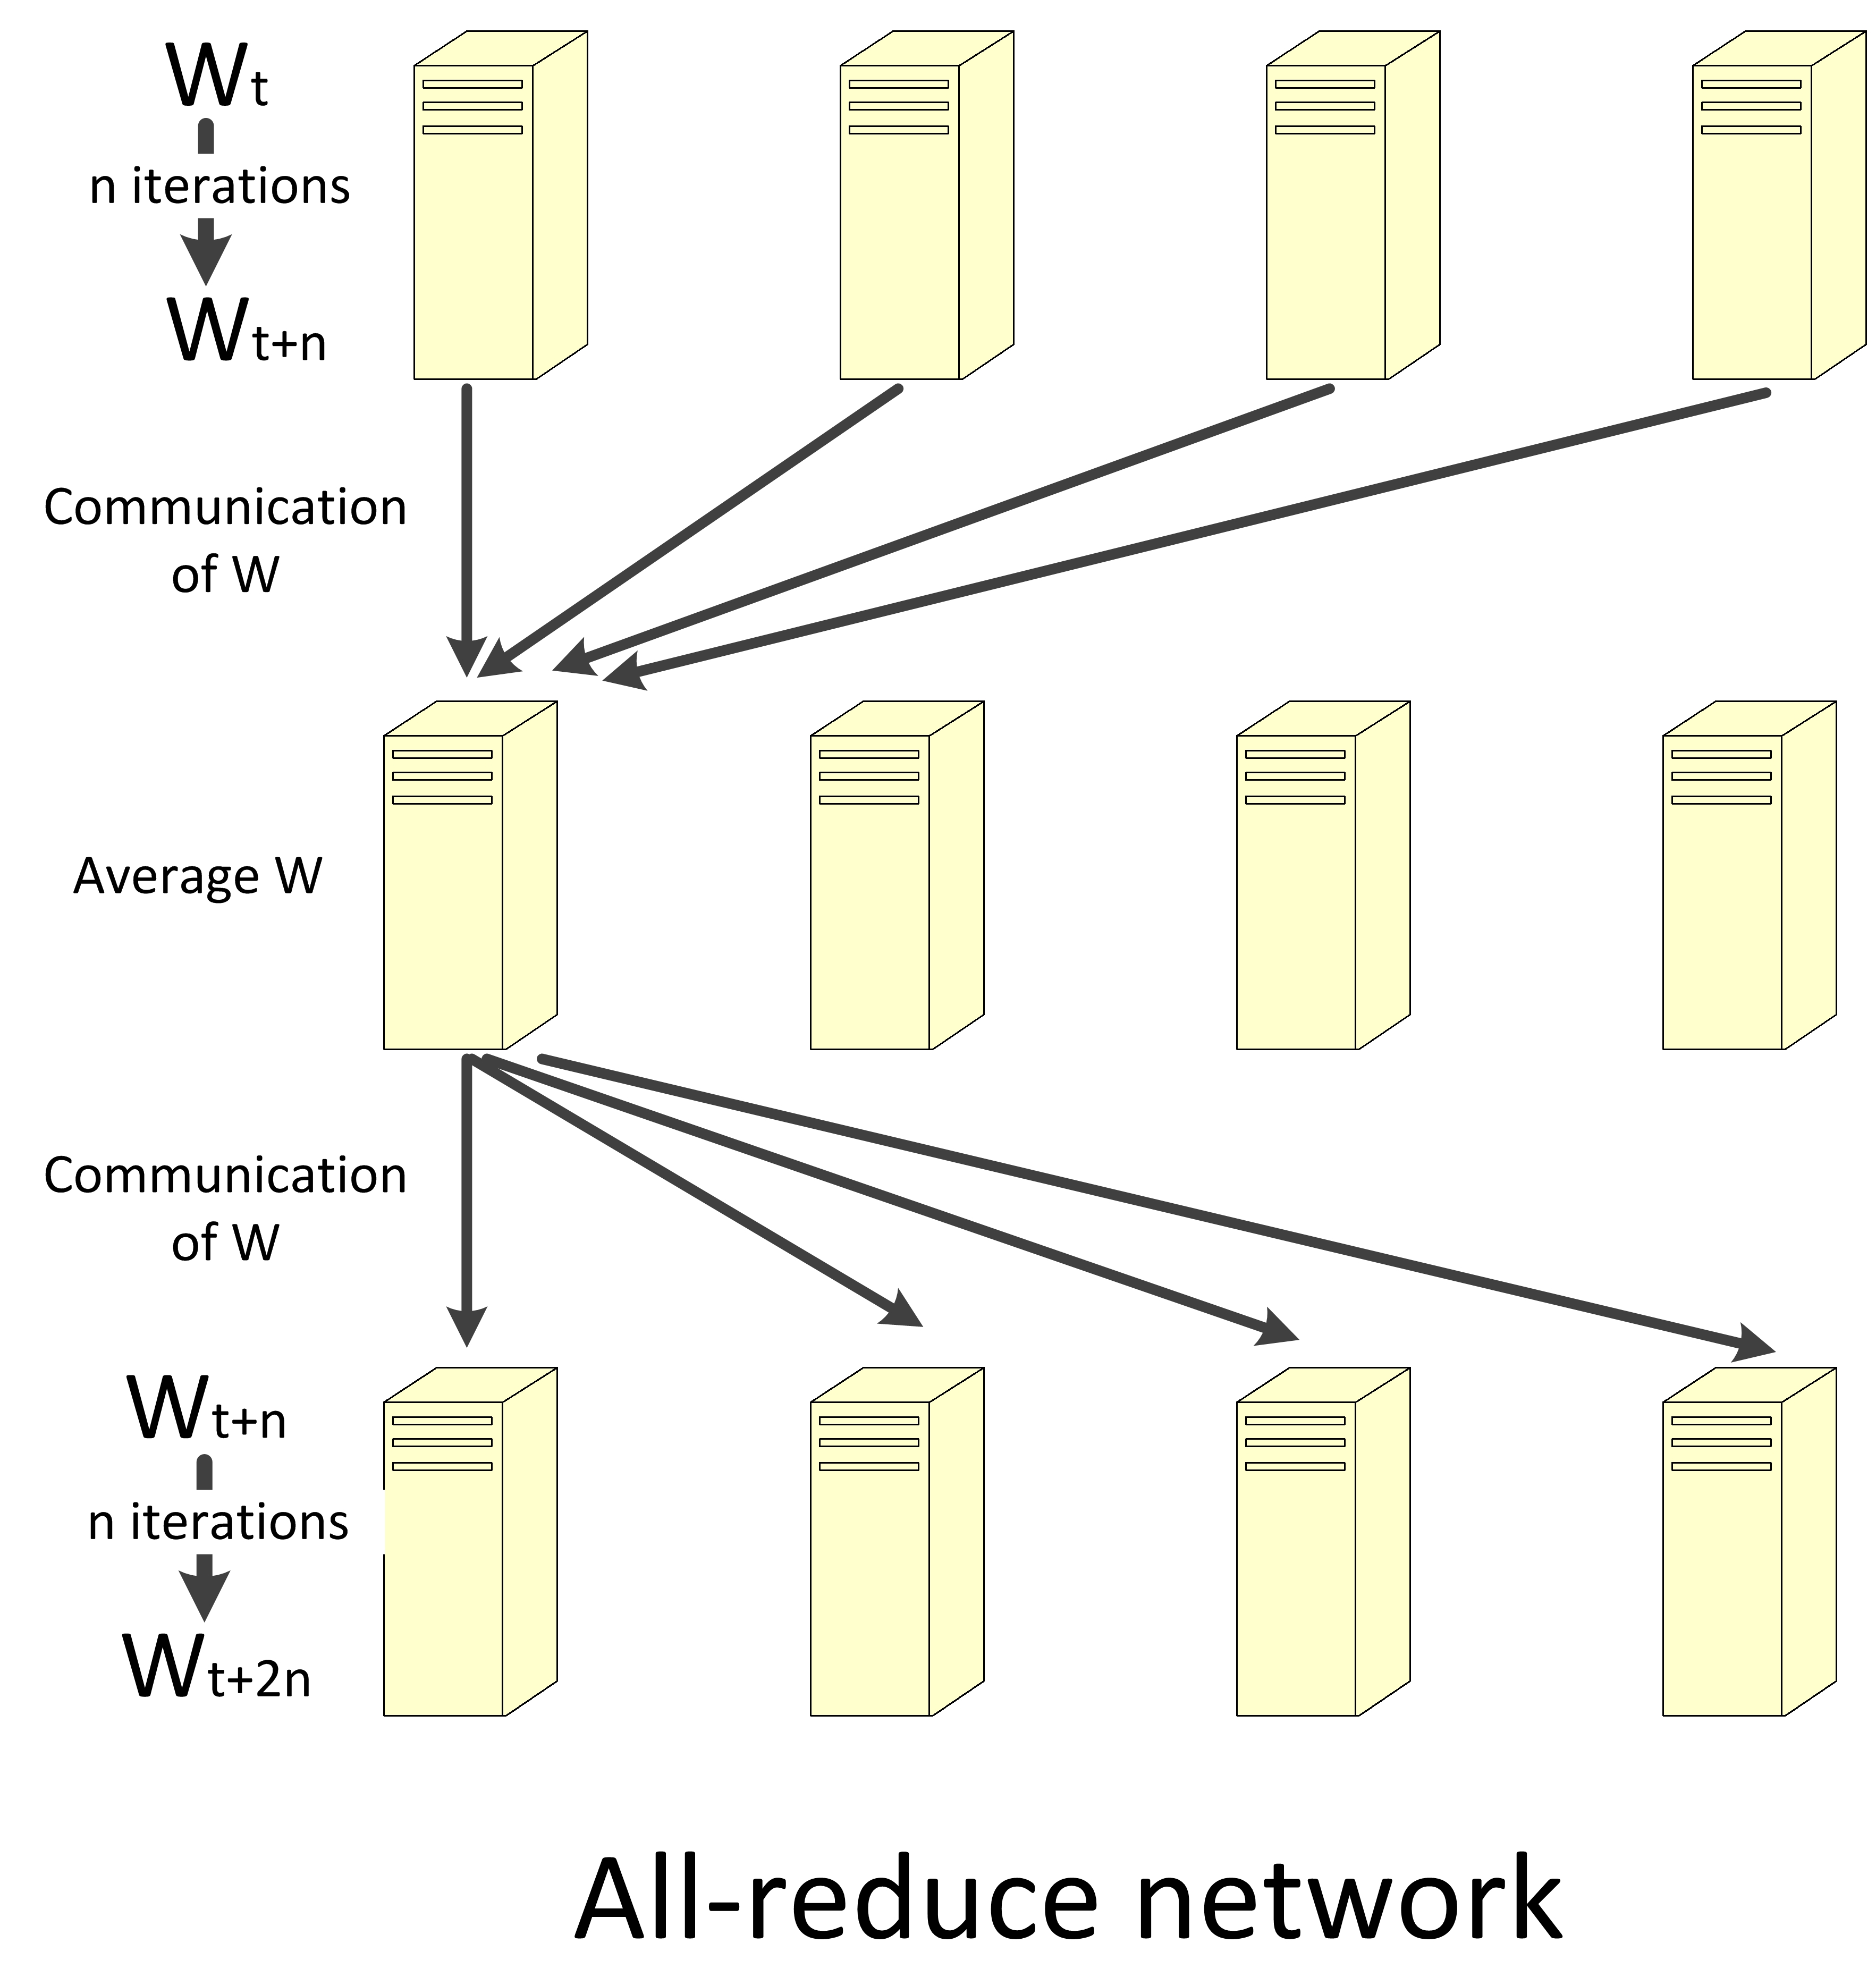
\includegraphics[width=0.35\textwidth]{allreduce.jpg}
    \caption{All-reduce network}
\end{figure}
\subsection{Butterfly Mixing}
 
Zhao and Canny (2012) proposed the butterfly mixing strategy. The butterfly mixing can reduce the communication for each iteartion: one node would only send and recieve message from one other node. But their communication orders are changed so that information for the whole network still can be spread to all nodes. Fig.~3 is an example of butterfly mixing with 4 nodes. The communication of butterfly mixing is bounded by the lantency. And butterfly mixing only require once communication to collect and average the weight, it does not need to send the averaged weight. Thus, the butterfly mixing has much less communication amount than all-reduce strategy. However, one node at butterfly mixing network only collect partial information from the network, its averaged weight can only reflect the information from two nodes. It takes $log(number of nodes)$ communication times to spread the message to the whole network. Thus, the converge speed of butterfly mixing is slower than all-reduce strategy. 
\begin{figure}[h!]
  
  \centering
    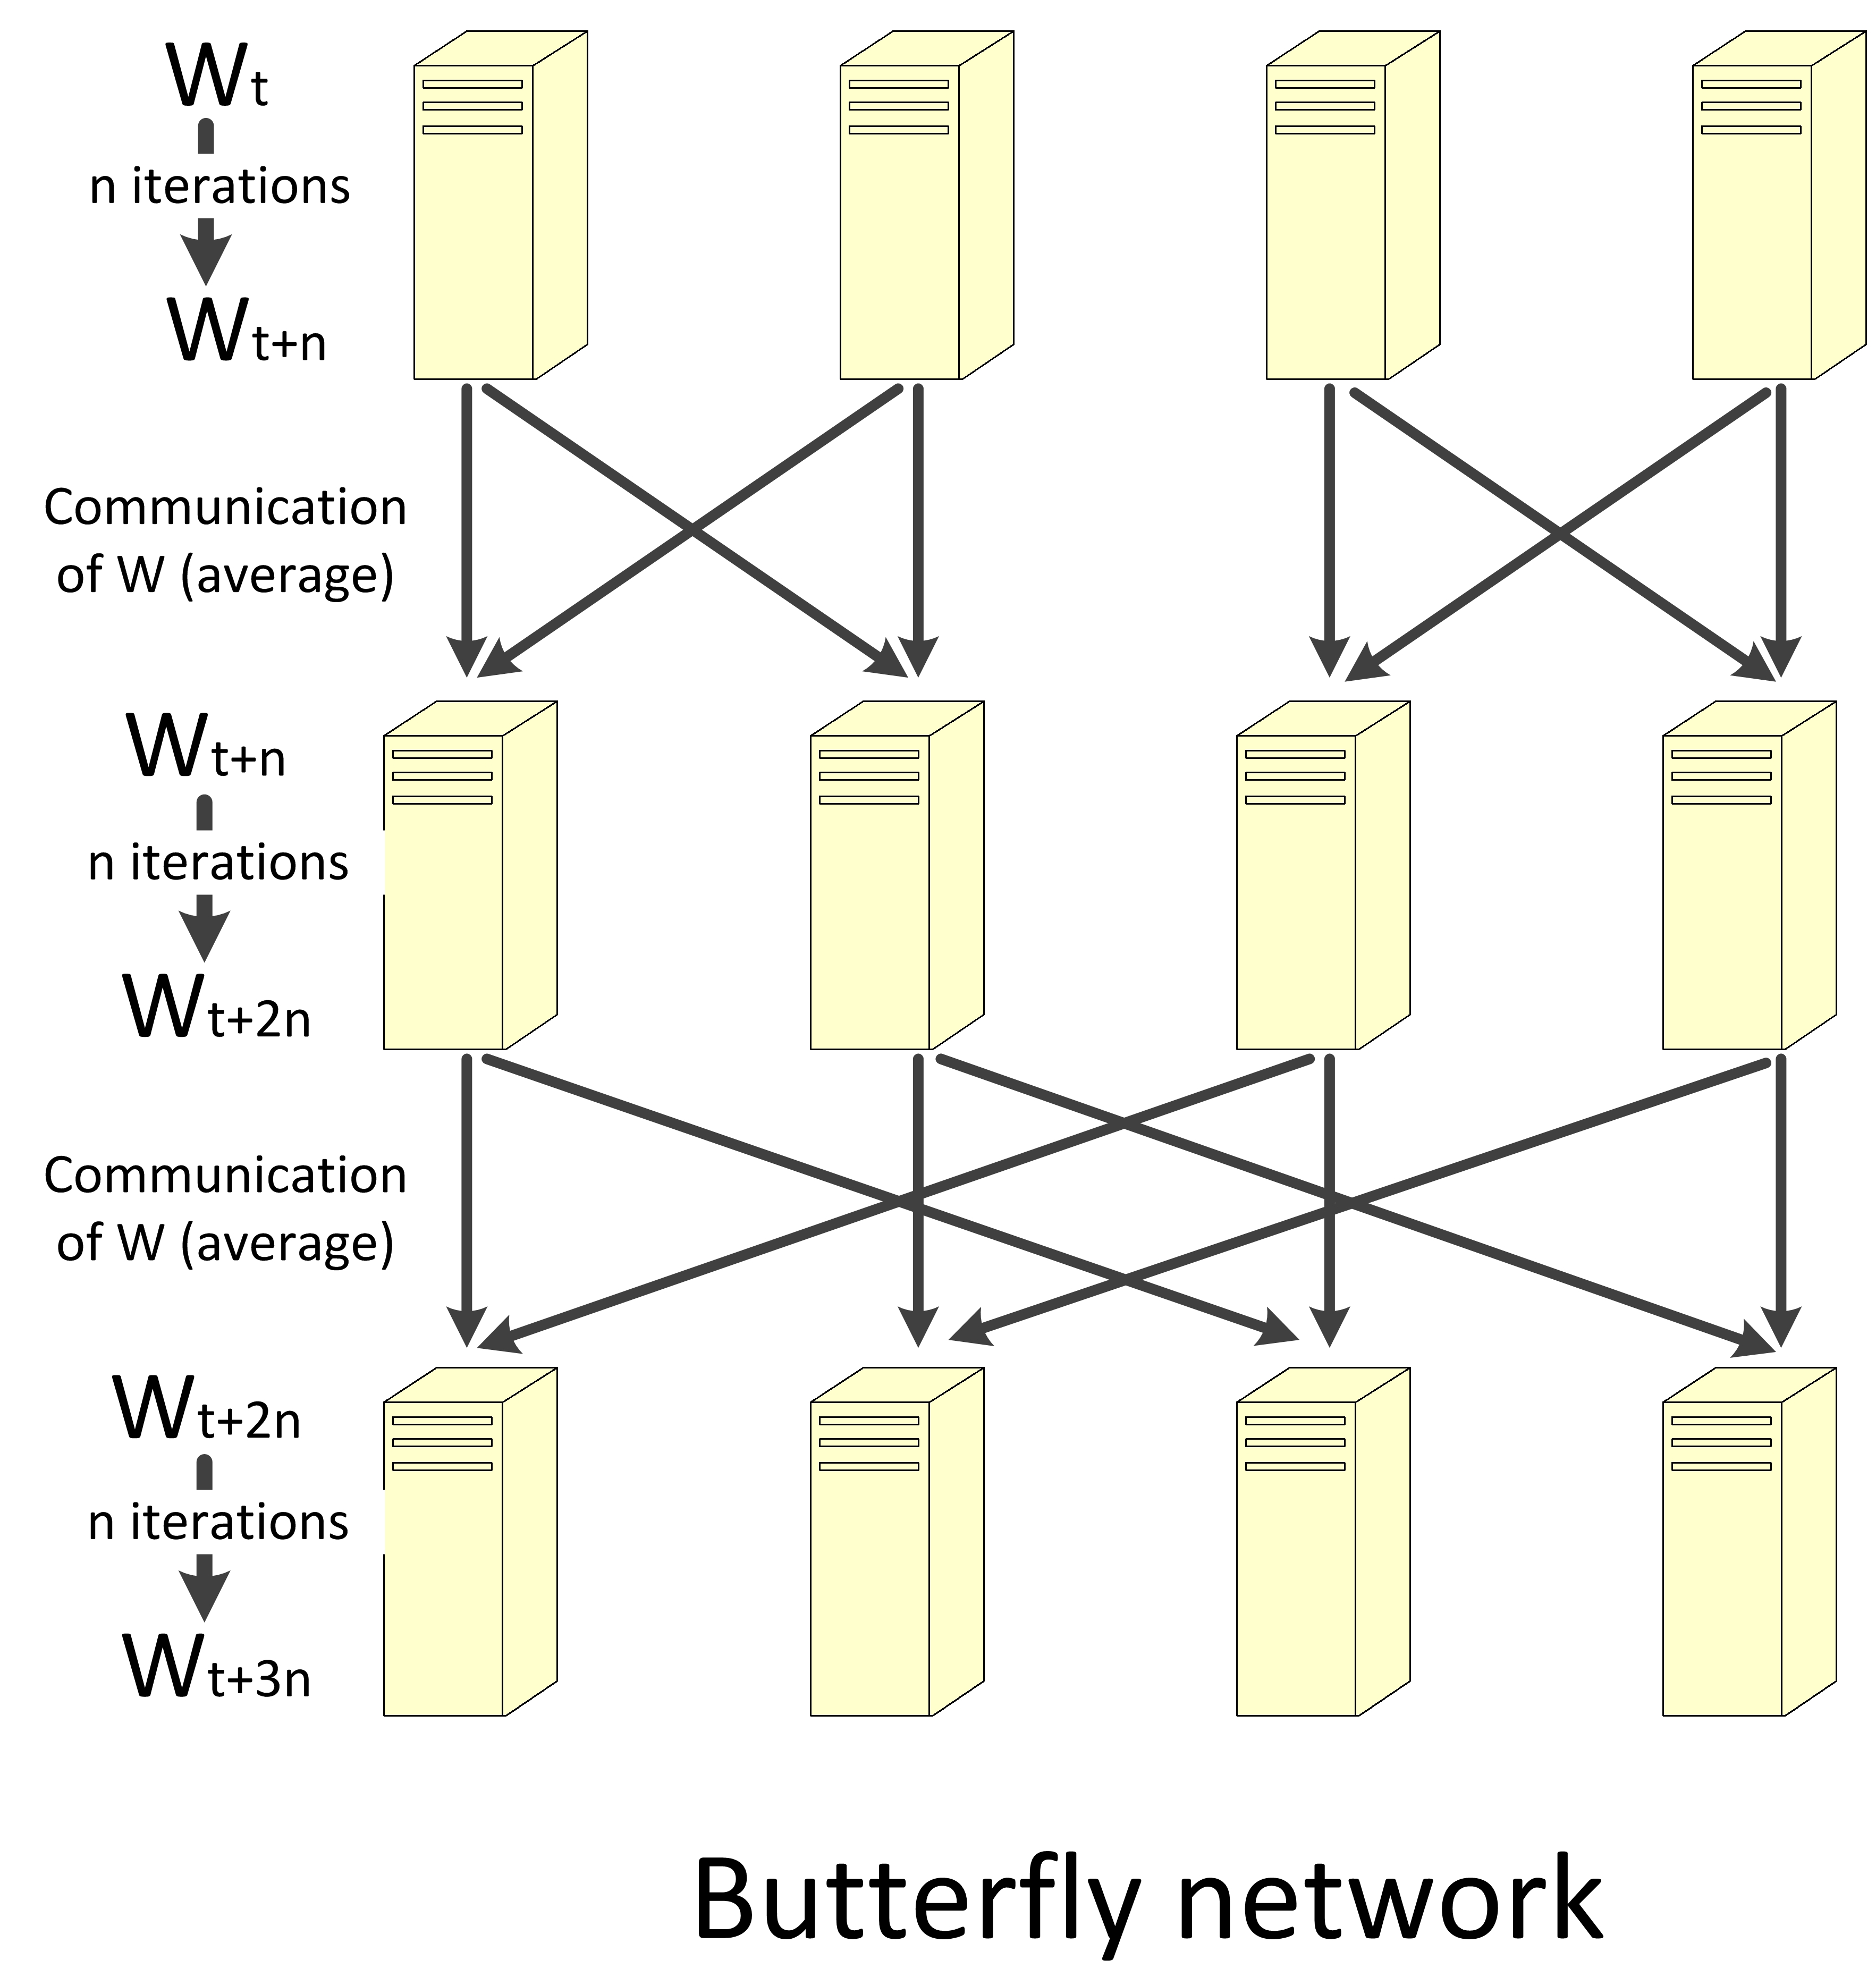
\includegraphics[width=0.35\textwidth]{butterfly.jpg}
    \caption{Butterfly mixing network.}
\end{figure}


\section{Experimental Results}
In this section, the all-reduce and butterfly mixing strategies are applied to train DNN for digit recognition task. The data I used is from THE MNIST DATABASE of handwritten digits. 
\subsection{Experiment setup}
The number of hidden layers in the NN is 2. In order to make a fair comparison, I fixed the training batch size (i.e. 20), initial step size (i.e. 1.0), learning rate (i.e. learning step decrease with $iteration^{0.75}$), and other parameters except the number of nodes ($n$), the number of updates between two consequential communications ($n_c$), and communication strategies (i.e. all-reduce or butterfly mixing). I will vary the number of nodes for $n = 4, 8, 16$, and the number of updates between two consequential communication for $n_c = 1, 8, 16$ For the initial weights, I only initialize it randomly once, and save it on the disk. Then for each experiment, they will read the same initial weight matrix from the disk. Because for each iteration at each node, it will randomly sample a batch of training data from the data set, there is some variance for our results. For each trail, I run six repeat experiment and compute their mean to decrease the randomness of the results. 

I design two kinds experiments. For the first category, I fix the total number of data points which are used to train (i.e. 80000 data points). For example, if there are 4 nodes in the system, I will run 1000 iterations for each node (i.e. $1000*4*20 = 80000$). If the convergence of butterfly in this kind of experiments is similar as the single node situation, distributed system is extremeley valuable to build to speed up the training process. That is to say, this category is the perfect situation for parallel distributed system (this category also corresponds to the strong scaling case when measuring parallel scaling performance).\\

For the second category, I fix the total number of iterations (i.e. 1000 iterations). For example, if there are 16 nodes, in the system, I will still run 1000 iteartions for each node. This category is like a worest situation for parallel system. If the convergence of butterfly mixing is worse than that of the single node, it is not worth to implement a parallel distributed system, since the parallel system will spend the same time as the single node with even worse accuracy (this category also corresponds to the weak scaling case when measuring parallel scaling performance).


\subsection{Fixed the training data size}

In this section, the convergence of the first category experiments is compared. Fig.~4 records the data with 4 nodes. Fig.~5 records the data with 8 nodes, and Fig.~6 for 16 nodes. In these figures, the horizontal axis is the number of used data points, and the vertical axis is the total cost on the whole data set. I use the dash line to represent the single node results, which is our comparison baseline. The blue curve represents the allreduce strategy, and the red curve represents the butterfly mixing strategy. On each subfigure, there are three curves, which represent the $n_c = 1 , 8 , 16$. \\

From the results, we find that for all cases, the single node curve (baseline case) is blow the other curves. Thus, no matter which communication strategies we choose, the weights in the distributed system converges slower than that in the single node system, if we fix the size of total training data. 

\begin{center}
\begin{figure*}
  
  \centering
    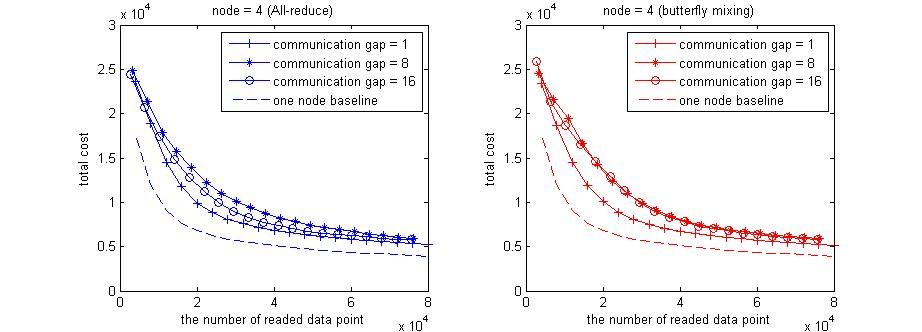
\includegraphics[width=0.9\textwidth]{batch20_node4_fixData.jpg}
    \caption{fixed training data size, $n=4$}

\end{figure*}
\end{center}

By comparing the curves with different $n_c$, we find that the smaller $n_c$, the faster convergence, because in smaller $n_c$ situation, the frequency of communication is high. However, we find the difference among curves with different $n_c$ for butterfly mixing strategy is much smaller than that for all-reduce. Thus, buttefly mixing is more robust for multiple nodes than all-reduce. \\  

We compared the convergence speed between all-reduce and butterfly mixing, and find that their convergence speed is similar. Butterfly mixing's converge speed is slight slower than that of all-reduce, but the difference is not significant. \\

In sum, if we fix the size of total train data, both all-reduce and butterfly mixing's performance is worse than that of single node. However, the difference of converge speed between all-reduce and butterfly mixing is small.
\begin{figure*}
  
  \centering
    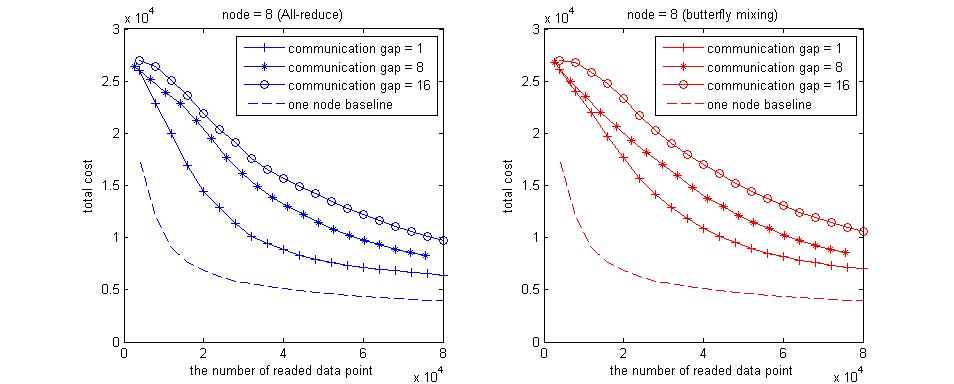
\includegraphics[width=0.9\textwidth]{batch20_node8_fixData.jpg}
    \caption{fixed training data size, $n=8$}
\end{figure*}
\begin{figure*}
  
  \centering
    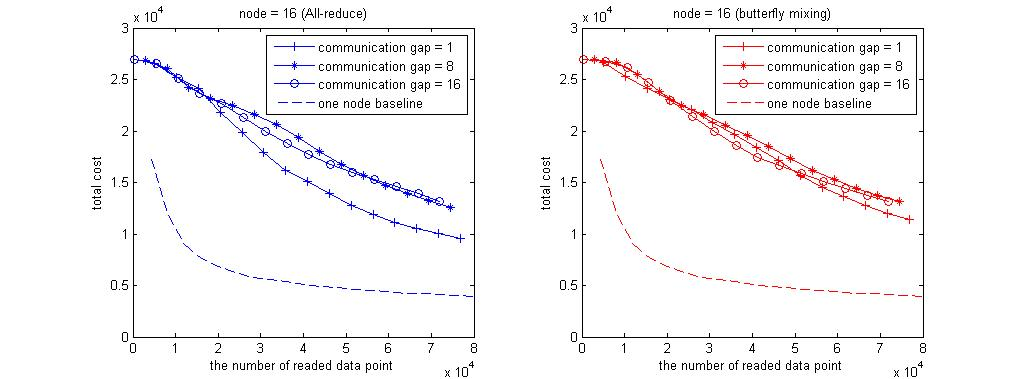
\includegraphics[width=0.9\textwidth]{batch20_node16_fixData.jpg}
    \caption{fixed training data size, $n=16$}
\end{figure*}


\subsection{Fixed the number of iteration}

In this section, we illustrate the results with fixed number of iterations. The results are shown in Fig.~7 -9. The horizontal axis is the number of iterations, and the vertical axis is the total cost on the whole data set. Similar as the previous section, there are 3 sets of results with $n = 4, 8, 16$. On each set, there are 4 curves, which are baseline, $n_c = 1, 8, 16$. Blue curves represent the all-reduce case, and red curves represent the butterfly mixing case. \\

In all the cases, the converge speed of distributed system is faster than that of single node. With the larger communication gap, the converge speed diminishes. \\

Comparing the all-reduce and the butterfly mixing, their converger speeds are similar. And butterfly mixing has more benefits when the communication gap is larger than 1 (i.e. when we don't reduce at each iteration). The difference among the curves with different gaps is much smaller for butterfly mixing than that for all-reduce. \\

In sum, if we fix the number of iterations, both the butterfly mixing and all-reduce have higher converge speed than single node. For the case $n_c > 1$, the butterfly mixing has faster converge speed than all-reduce. The effects of $n_c$ to converge speed for butterfly mixing is smaller than that for all-reduce. 


\begin{figure*}
  
  \centering
    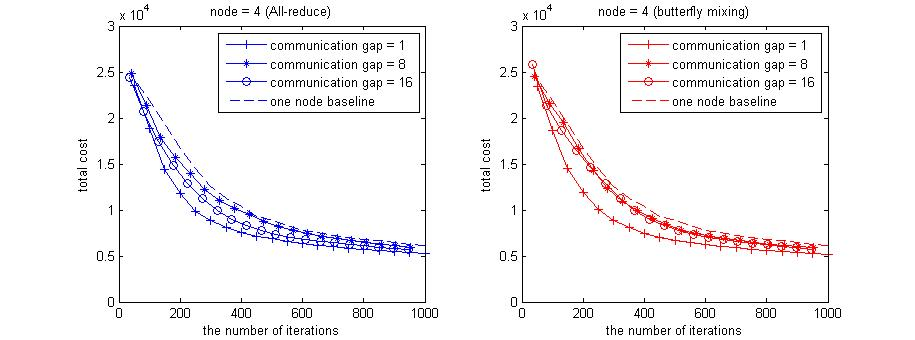
\includegraphics[width=0.9\textwidth]{batch20_node4_fixIter.jpg}
    \caption{Fix iteration number, $n = 4$}
\end{figure*}

\begin{figure*}
  
  \centering
    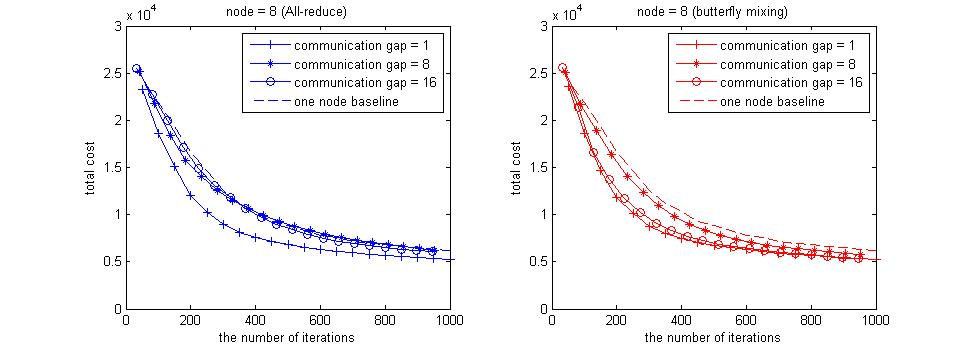
\includegraphics[width=0.9\textwidth]{batch20_node8_fixIter.jpg}
    \caption{Fix iteration number, $n = 8$}
\end{figure*}
\begin{figure*}
  
  \centering
    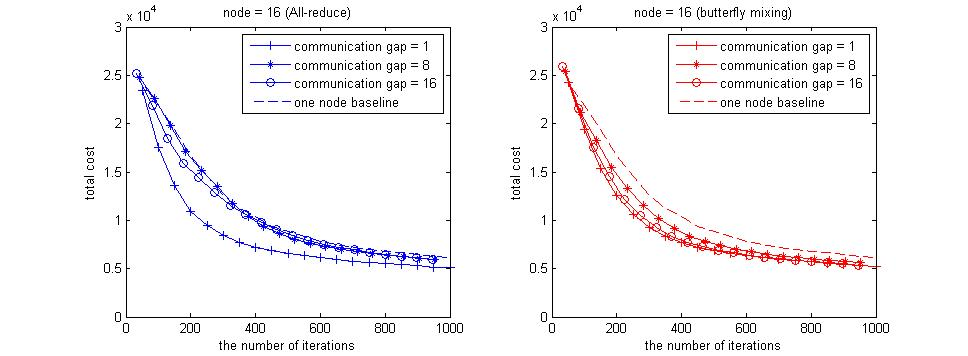
\includegraphics[width=0.9\textwidth]{batch20_node16_fixIter.jpg}
    \caption{Fix iteration number, $n = 16$}
\end{figure*}

\section{Conclusion}

In this project, I implement a nerual network and a framework which can simulate the distributed system. I use the framework to simulate training the NN with multiple nodes. Two communication strategies' converge speed are compared here: all-reduce and butterfly. This study can be a preliminary research before implementing a real distributed system.\\

From the simulation data I find that if I fix the size of total training data, both all-reduce and butterfly mixing have slower converge speed than single node. But if I fix the iteration number, both all-reduce and butterfly mixing have higher convergence speed than single node. Thus, building a distributed system to train NN may bring benefits. \\

By comparing the convergence speed between all-reduce and butterfly mixing, butterfly mixing has advantages when the gap between two communication is larger than one iteration.  


% References should be produced using the bibtex program from suitable
% BiBTeX files (here: strings, refs, manuals). The IEEEbib.bst bibliography
% style file from IEEE produces unsorted bibliography list.
% -------------------------------------------------------------------------
\bibliographystyle{IEEEbib}
\bibliography{paper}

\end{document}
